% !TeX root = Features.tex
\documentclass[../Dissertation.tex]{subfiles}

\begin{document}

\section{Feature Overview}
A software application was developed from the outlined design specification. This application is composed of two decoupled subsystems. The first of these subsystems is concerned with the generation and composition of Petri nets, and is an implementation of the theory outlined in Section \ref{sec:towardsatool}. Thus, the focus of the second subsystem is visualisation and user interaction.

\subsection{Types to Petri nets, an implementation}
A C\lstinline{++} library was created for the generation and composition of Petri nets. This library also includes parsing procedures for types. This library does not include any computation involving the graphical user interface, and may be used independently in other software applications.
\par
The generation of a Petri net model using the C\lstinline{++} library, requires two strings as input. These strings correspond to a System $F_\kappa$ type and a naturality type. Accordingly, the input strings must be generated by the grammars depicted in Figures \ref{fig:typegrammar} and \ref{fig:natgrammar}, respectively. The strings are parsed into an appropriate abstract syntax tree (AST). The constructed AST is used to generate an in-memory representation of a Petri net, for each type variable occurring within the input type.
\par
In a deviation from the design specification, the default naturality type maps every type variable to 0, and not 1. Furthermore, the input string for a naturality type indirectly defines a function, by describing which type variables are to be equated. For example, an input naturality type of \lstinline{0 2 => 0 2} does not describe two functions which map their first type variable to 0, and their second to 2. Rather, both of the functions defined by this naturality type are defined as $n \mapsto n$. Intuitively, the numbers are unique identifiers, which indirectly describe a function.
\par
Composition requires two Petri nets as input. The generation of a composite follows from Definition \ref{def:petricomposition}. As before, only an in-memory representation of the composite Petri net is created, which can be used in further operations.
\par
A separate interface layer, created using the N-API library, was developed for interoperating with a Typescript application. The interface layer transforms an in-memory C\lstinline{++} representation of a Petri-net into a Typescript object. This object provides a referentially transparent interface, i.e., the Typescript interface only exposes non-mutating functions, which compute the same value given the same input. Notably, the Typescript interface includes a function which takes a type variable as input, and returns the corresponding Petri net as a Typescript object.

\subsection{Visualisation and the user interface}
Upon opening the desktop GUI application, a user is presented with a blank workspace. Adding a new component to the workspace, or deleting an existing one, requires the use of a keyboard shortcut. The complete list of available keyboard shortcuts is presented in Figure \ref{fig:shortcuts}.

\begin{figure}[H]
\begin{center}
\begin{tabular}{l l}
\keystroke{\cmd/\ctrl} + \keystroke{n} & Add a new component to the workspace.\\\\
\keystroke{\cmd/\ctrl} + \keystroke{d} & Delete the most recently selected component.\\\\
\keystroke{\cmd/\ctrl} + \keystroke{.} & Compose the selected components.\\\\
\keystroke{\cmd/\ctrl} + \keystroke{s} & Save the primary selected Petri net to PNG/SVG.\\\\
\keystroke{\cmd/\ctrl} + \keystroke{e} & Export the primary selected Petri net to Latex (Tikz-cd).
\end{tabular}
\end{center}
\caption{Keyboard shortcuts within the application.}
\label{fig:shortcuts}
\end{figure}

In Figure \ref{fig:component} a single component is shown within the application. The transformation \lstinline{(a -> a)} \lstinline{=> a} has been entered into the input field on the top-left. The default naturality type has been automatically generated and presented in the bottom-left input field. The type variable \lstinline{a} has been provided, and the corresponding Petri net has been generated under the input interface. The graph is automatically updated upon any change in the input. As required by the outlined design, an enabled transition can be fired simply by clicking it.
\par
The component can be moved, within the workspace, by holding down the left mouse button over the grey handle, and then moving the mouse. Holding down the left button, while the mouse is located in the space surrounding the Petri net, and then moving the mouse, will translate the graph in its local frame. Scrolling upwards, while the mouse is located in the local frame of a Petri net, will zoom in, while scrolling downwards will zoom out.

\begin{figure}[H]
\begin{center}
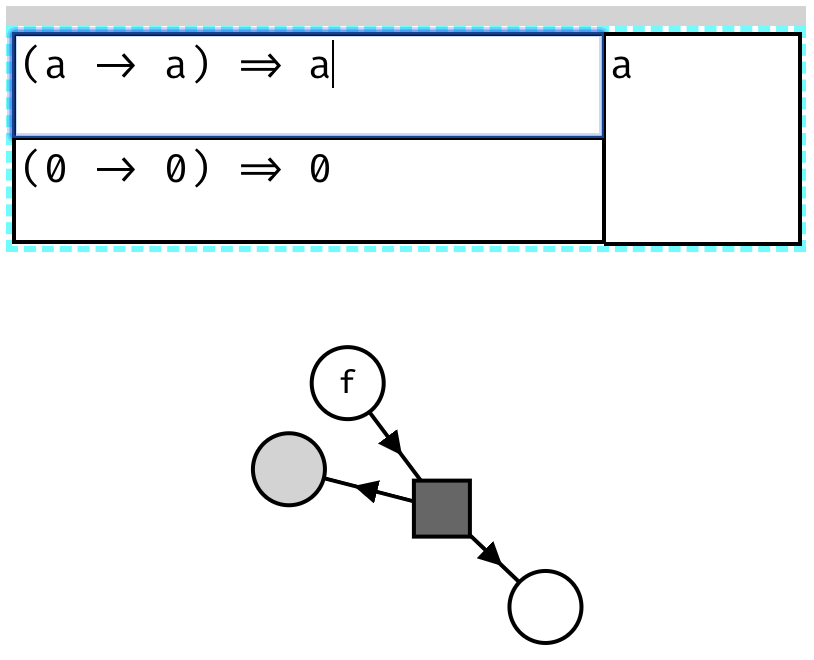
\includegraphics[scale=0.45]{component}
\end{center}
\caption{A single, selected component.}
\label{fig:component}
\end{figure}

There are two notable features of this component, which were not considered in the original design. The first is the presence of a dashed cyan border around the input. This border is used to identify the `primary' selected component. The notion of `primary' and `secondary' selection will be expanded upon shortly.
\par 
The second feature, not outlined in the original design, is the ability to drag individual nodes of the Petri net. This interactive feature provides a means by which a user can re-arrange and rotate the graph. Note that the partitioning of place nodes is preserved, such that the involved functors remain discernible. This grouping of place nodes is apparent in the provided examples.
\par
Demonstrating composition requires the addition of a second component to the workspace. In Figure \ref{fig:selection}, a second component is shown to have been created in the workspace. Observe that one component has a dashed purple border surrounding its input. This is used to identify the `secondary' selected component. 
\par
A maximum of two components can be selected at any time. Hovering the mouse over a component and then clicking the left mouse button will set the `primary' selection. Setting the `primary' selection will clear all existing selections. Once a `primary' selection has been made, holding down the shift key while clicking the left mouse button can be used to make a `secondary' selection. The keyboard shortcut for deletion will only delete the most recently selected component.

\begin{figure}[H]
\begin{center}
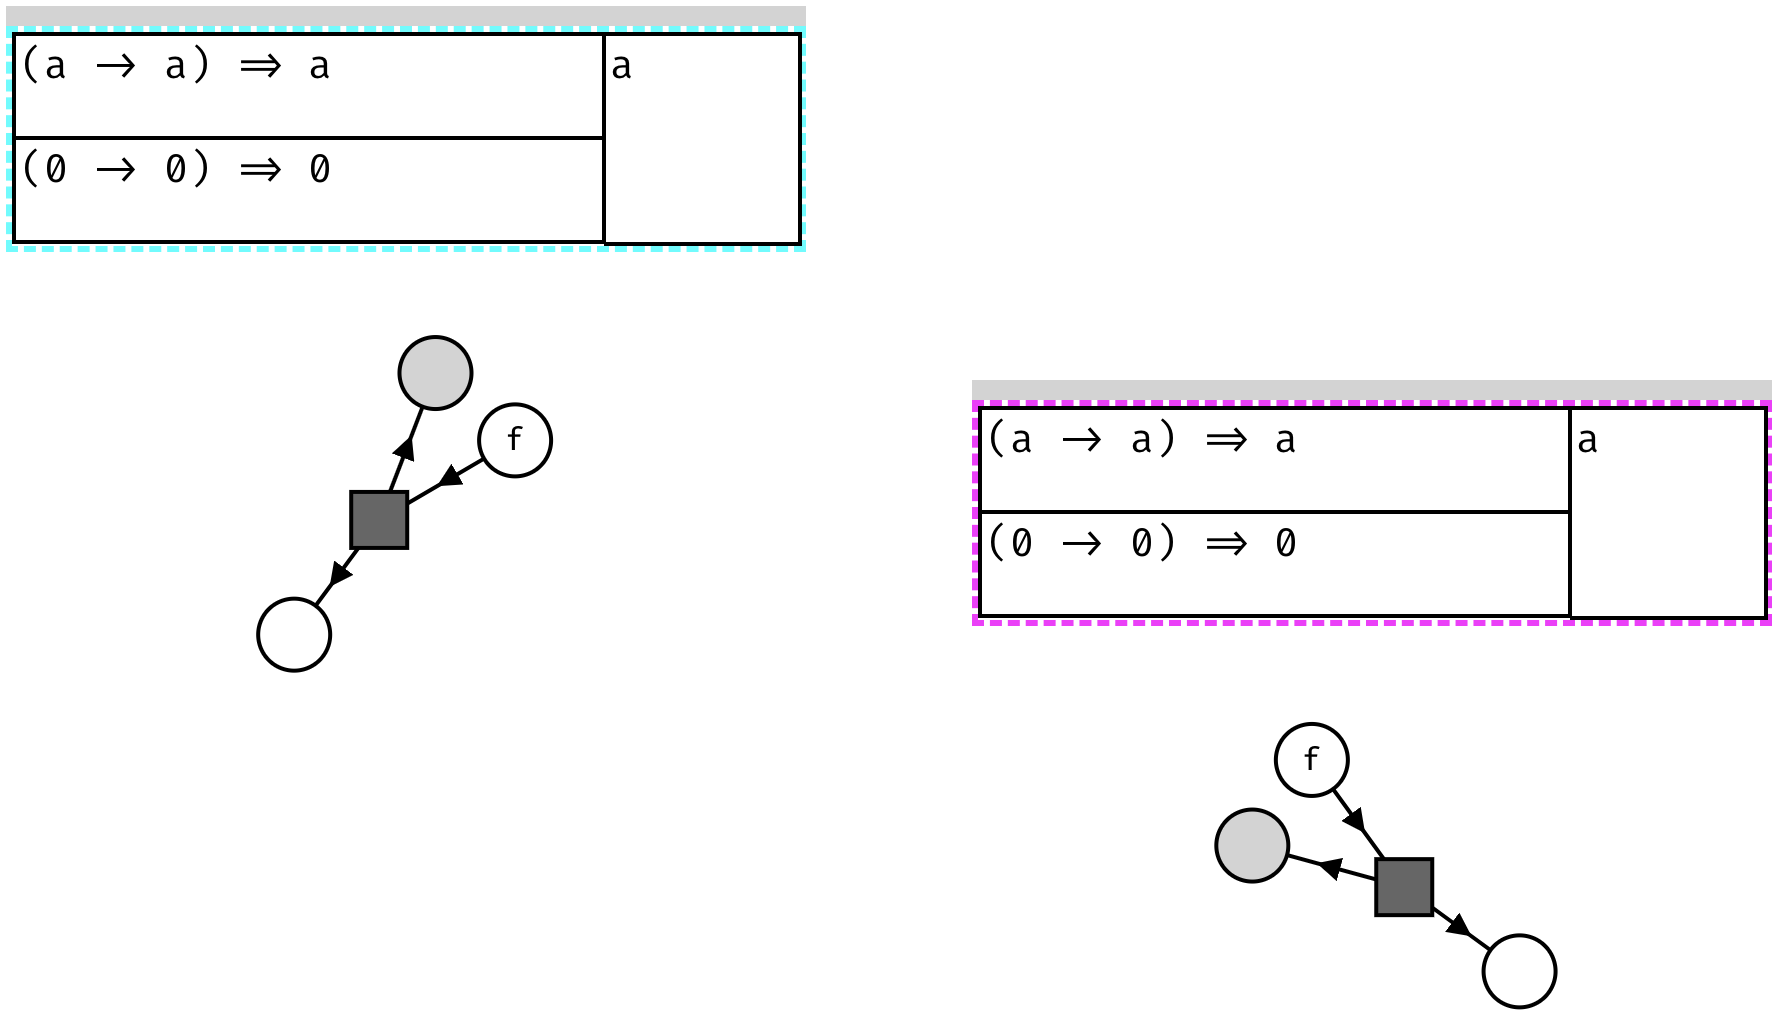
\includegraphics[scale=0.45]{selection}
\end{center}
\caption{Two selected components.}
\label{fig:selection}
\end{figure}

The order of `selection' is in direct correspondence with the order of composition. The keyboard shortcut for composition will compose the `secondary' selection with the `primary' selection, i.e., `secondary' after `primary'. The composition of two selected components, within the application, is shown in Figure \ref{fig:compose1}. Composition is only possible if the codomain of the `primary' selection is unifiable with the domain of the `secondary' selection. In the current version of the application, failed composition is simply ignored.
\par
Components generated by composition feature two key differences from those which are not. The type field is not editable, and the naturality type is not displayed. The type variable may still be changed in order to display the Petri net corresponding to each variable.
\par 
The in-memory representation of a composite type preserves the composition boundary. Changing the domain or codomain of the generated composite type has the potential to render the composition boundary invalid. Consequently, permitting modification of the type of a composite component, is not a sensible operation. This same reasoning applies to permitting modification of the naturality type. However, a read-only naturality type would simply provide redundant information, already depicted by the graph, and is therefore not displayed.

\begin{figure}[H]
\begin{center}
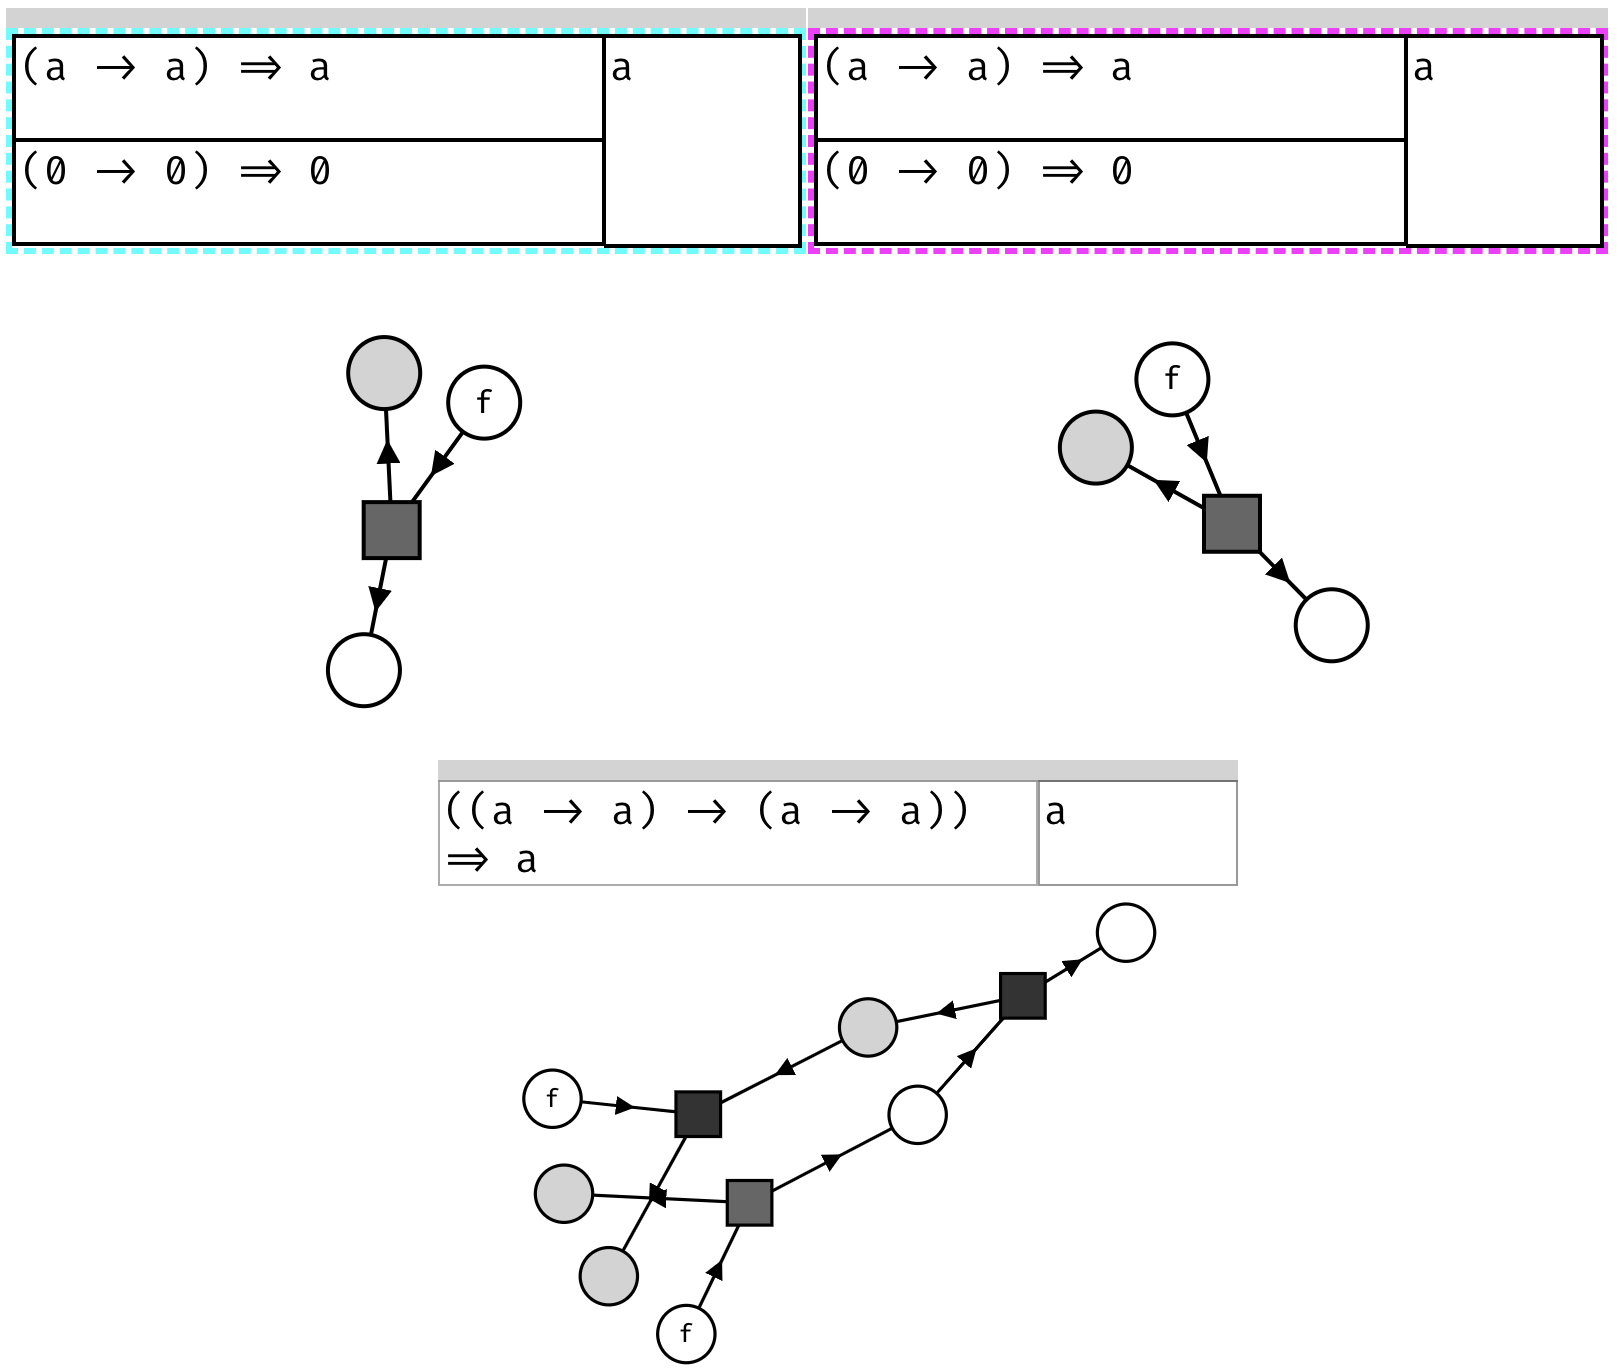
\includegraphics[scale=0.45]{compose1}
\end{center}
\caption{Two selected components and their composition.}
\label{fig:compose1}
\end{figure}

Recall the \lstinline{applyToFirst :: (a -> a, a, a)} \lstinline{-> (a, a)} function, first introduced in Listing \ref{Haskell-ParametricityFail}. A Petri net, corresponding to the naturality condition of \lstinline{applyToFirst}, was given in Figure \ref{fig:applyToFirstBetter}. The generation of this Petri net required defining a particular naturality type. Figure \ref{fig:applytofirstimg} demonstrates the modification of a naturality type, within the application, to generate a Petri net corresponding to the naturality condition of \lstinline{applyToFirst}. 
\par
As previously recognised, the implementation of \lstinline{applyToFirst} may be given the more general type \lstinline{(a -> b, a, c)}  \lstinline{-> (b, c)}. The Petri net for this type was depicted in Figure \ref{fig:applyToFirstLast}. Within the developed application, the naturality condition of each type variable is viewed separately. Each of the Petri nets generated by \lstinline{(a -> b, a, c)}  \lstinline{-> (b, c)}, and additional examples involving transformations with multiple type variables, are presented in Appendix \ref{app:differentvars}.

\begin{figure}[H]
\begin{center}
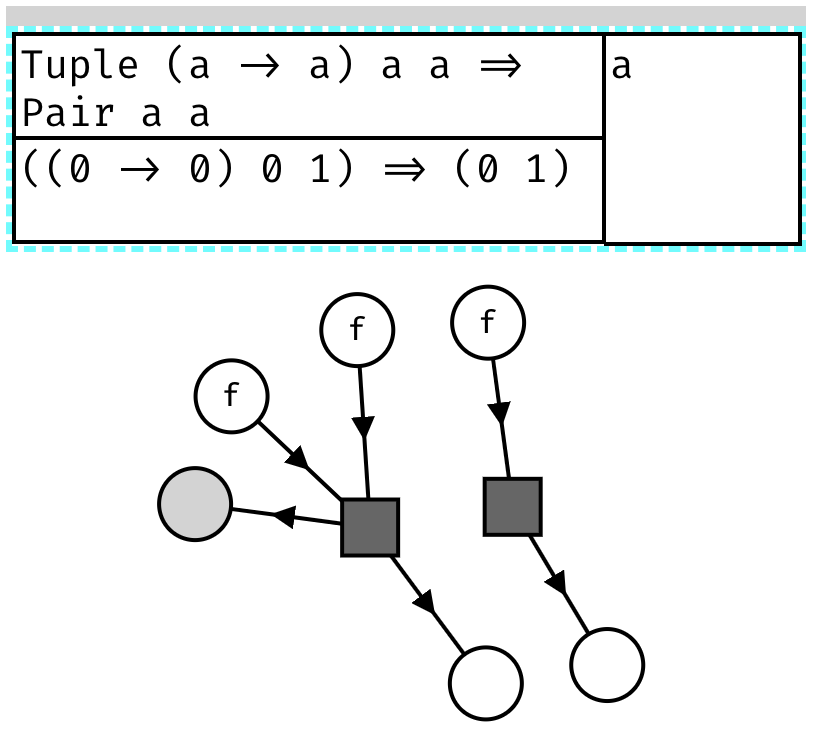
\includegraphics[scale=0.45]{applytofirst}
\end{center}
\caption{Petri net generated for naturality condition of \lstinline{applyToFirst}.}
\label{fig:applytofirstimg}
\end{figure}

A composite component can continue to be composed with any other component, with the usual condition that their types must unify. Iterated composition, within the application, is shown in Appendix \ref{app:itcomp}. Examples demonstrating the composition of Petri nets, with modified naturality types, are given in Appendix \ref{app:modcomp}. Examples of the zoom and translation features are given in Appendix \ref{app:zoomtrans}.

\subsection{Image and LaTeX exporting}
Petri nets generated within the application can be exported to a range of external data formats. This includes the ability to save a Petri net as an image in either the portable network graphics (PNG) or scalable vector graphics (SVG) format.
\par
Image formats are less suitable for research papers, where high-quality graphs can be generated with the typesetting system of LaTeX. For the purpose of improving the utility of the application for research purposes, Petri nets can also be exported to LaTeX. The exported LaTeX requires the `tikz-cd' package. This feature will be used extensively in demonstrating the results attained by use of the application.

\end{document}